\documentclass[a4paper]{article}

\def\nbook {All of Statistics: A Concise Course in Statistical Inference}
\def\nbookshort {All of Statistics}

% Shared preamble. The fallback lets the document build whether the working
% directory is its own folder or the project root.
\IfFileExists{header.tex}{\input{header}}{%%%%%%%%%%%%%%%%%%%%
% AUTHOR AND HEADER
% define \nbook
%%%%%%%%%%%%%%%%%%%%

\makeatletter
\ifx \nauthor\undefined
  \def\nauthor{David A. Lee}
\else
\fi

\author{\nbook \\ \small Solutions by \nauthor}
\date{}

%%%%%%%%%%%%%%%%%%%%
% PACKAGES
%%%%%%%%%%%%%%%%%%%%

\usepackage{alltt} 
\usepackage{amsfonts}
\usepackage{amsmath}
\usepackage{amssymb}
\usepackage{amsthm}
\usepackage{bm}
\usepackage{booktabs}
\usepackage{caption}
\usepackage{centernot}
\usepackage{enumitem}
\usepackage{fancyhdr}
\usepackage[T1]{fontenc}
\usepackage{graphicx}
% Images live in chap1/ ... chap8/ at the project root, while the documents that
% use them sit one level down (allofstats/, allofstatschap1/, ...). Listing both
% "./" and "../" lets a document keep writing \includegraphics{chap1/foo.eps}
% and still resolve it whether it is compiled from its own folder or from the
% project root.
\graphicspath{{./}{../}}
\usepackage{mathdots}
\usepackage{mathtools}
\usepackage{microtype}
\usepackage{multirow}
\usepackage{pdflscape}
\usepackage{pgfplots}
\pgfplotsset{compat=1.18}
\usepackage{siunitx}
\usepackage{slashed}
\usepackage{tabularx}
\usepackage{tikz}
\usepackage{titletoc}
\usepackage{tkz-euclide}
\usepackage[normalem]{ulem}
\usepackage{url}
\usepackage[all]{xy}
\usepackage{imakeidx}

% fonts
% use \textsf to change to Computer Modern Bright
\renewcommand{\sfdefault}{cmbr} % keeps default font Computer Modern Roman

% makeindex for table of contents
\makeindex[intoc, title=Index]
\indexsetup{othercode={\lhead{ Index }}}

% table of contents remove numbering
\setcounter{secnumdepth}{0}

% pagestyle
\pagestyle{fancyplain}

% header
\lhead{	\nouppercase{\leftmark} }
\ifx \nextra \undefined
  \rhead{
    \ifnum\thepage=1
    \else
      \nbookshort \  | \nauthor
    \fi}
\else
  \rhead{
    \ifnum\thepage=1
    \else
      \nbookshort (\nextra)
    \fi}
\fi

% proof environment

\newcommand{\prooffont}{\scshape}
\usepackage{xpatch}
\tracingpatches
\xpatchcmd{\proof}{\itshape}{\prooffont}{}{}

% Python environment (for typesetting Python code)

% Default fixed font does not support bold face
\DeclareFixedFont{\ttb}{T1}{txtt}{bx}{n}{8} % for bold
\DeclareFixedFont{\ttm}{T1}{txtt}{m}{n}{8}  % for normal

% Custom colors
\usepackage{color}
\definecolor{deepblue}{rgb}{0,0,0.5}
\definecolor{deepred}{rgb}{0.6,0,0}
\definecolor{deepgreen}{rgb}{0,0.5,0}

\usepackage{listings}

% Python style for highlighting
\newcommand\pythonstyle{\lstset{
language=Python,
basicstyle=\ttm,
morekeywords={self},              % Add keywords here
keywordstyle=\ttb\color{deepblue},
emph={MyClass,__init__},          % Custom highlighting
emphstyle=\ttb\color{deepred},    % Custom highlighting style
stringstyle=\color{deepgreen},
frame=tb,                         % Any extra options here
showstringspaces=false
}}


% Python environment
\lstnewenvironment{python}[1][]
{
\pythonstyle
\lstset{#1}
}
{}

% Python for external files
\newcommand\pythonexternal[2][]{{
\pythonstyle
\lstinputlisting[#1]{#2}}}

% Python for inline
\newcommand\pythoninline[1]{{\pythonstyle\lstinline!#1!}}

%%%%%%%%%%%%%
% FUNCTIONS %
%%%%%%%%%%%%%

\DeclarePairedDelimiter\abs{\lvert}{\rvert}%
\DeclarePairedDelimiter\norm{\lVert}{\rVert}%

%%%%%%%%%%%%%%%%%%%%
% DOCUMENT GEOMETRY
%%%%%%%%%%%%%%%%%%%%

\ifx \ntrim \undefined
\else
  \usepackage{geometry}
  \geometry{
	  papersize={379pt, 699pt},
	  textwidth=345pt,
	  left=17pt,
	  top=54pt,
	  right=17pt,
  }
\fi

% maketitle statement
\title{}
\ifx \nisofficial \undefined
\let\@real@maketitle\maketitle
\renewcommand{\maketitle}{\@real@maketitle\begin{center}\begin{minipage}[c]{0.9\textwidth}\centering\footnotesize All errors, typographical and substantive, and other offenses, are entirely my own.\end{minipage}\end{center}}
\else
\fi

%%%%%%%%%%%%%%%%%%%%
% THEOREMS
%%%%%%%%%%%%%%%%%%%%

%\theoremstyle{definition}
\newtheorem*{axiom}{Axiom}
\newtheorem*{claim}{Claim}
\newtheorem*{conjecture}{Conjecture}
\newtheorem*{cor}{Corollary}
%\newtheorem*{dfn}{Definition}
\newtheorem*{eg}{Example}
\newtheorem*{ex}{Exercise}
%\newtheorem*{lemma}{Lemma}
\newtheorem*{prop}{Proposition}
%\newtheorem*{thm}{Theorem}
\newtheorem*{remark}{Remark}
\newtheorem*{warning}{Warning}

%%%%%%%%%%%%%%%%%%%%
% FORMATTING AESTHETICS
%%%%%%%%%%%%%%%%%%%%

% itemize bullets
\renewcommand{\labelitemi}{-}
\renewcommand{\labelitemii}{$\circ$}
\renewcommand{\labelenumi}{(\roman{*})}

% new page section
\let\stdsection\section
\renewcommand\section{\newpage\stdsection}

%%%%%%%%%%%%%%%%%%%%
% \mathbb commands
%%%%%%%%%%%%%%%%%%%%

\newcommand{\C}{\mathbb{C}}
\newcommand{\N}{\mathbb{N}}
\newcommand{\Q}{\mathbb{Q}}
\newcommand{\R}{\mathbb{R}}
\newcommand{\Z}{\mathbb{Z}}


%%%%%%%%%%%%%%%%%%%%
% Probability Operators
%%%%%%%%%%%%%%%%%%%%

\DeclareMathOperator{\Bernoulli}{Bernoulli}
\DeclareMathOperator{\betaD}{Beta}
\DeclareMathOperator{\bias}{\textsf{bias}}
\DeclareMathOperator{\binomial}{Binomial}
\DeclareMathOperator{\corr}{Corr}
\DeclareMathOperator{\cov}{\textsf{Cov}}
\DeclareMathOperator{\Exp}{Exp}
\DeclareMathOperator{\gammaD}{Gamma}
\DeclareMathOperator{\mse}{\textsf{MSE}}
\DeclareMathOperator{\multinomial}{Multinomial}
\DeclareMathOperator{\Poisson}{Poisson}
\DeclareMathOperator{\sd}{sd}
\DeclareMathOperator{\se}{\textsf{se}}
\DeclareMathOperator{\Uniform}{Uniform}
\newcommand{\Prob}{\mathbb{P}}
\newcommand{\var}{\mathbb{V}}
\newcommand{\E}{\mathbb{E}}

%%%%%%%%%%%%%%%%%%%%
% TCOLORBOX CODE FROM SeniorMars
%%%%%%%%%%%%%%%%%%%%

%\usepackage[varbb]{newpxmath} changes math font to newpxmath
\usepackage{xfrac}
\usepackage[makeroom]{cancel}
\usepackage{mathtools}
\usepackage{bookmark}
\usepackage{enumitem}
\usepackage{hyperref,theoremref}
\hypersetup{
	pdftitle={Assignment},
	colorlinks=true, linkcolor=doc!90,
	bookmarksnumbered=true,
	bookmarksopen=true
}
\usepackage[most,many,breakable]{tcolorbox}
\usepackage{xcolor}
\usepackage{varwidth}
\usepackage{varwidth}
\usepackage{etoolbox}
%\usepackage{authblk}
\usepackage{nameref}
\usepackage{multicol,array}
\usepackage{tikz-cd}
\usepackage[ruled,vlined,linesnumbered]{algorithm2e}
\usepackage{comment} % enables the use of multi-line comments (\ifx \fi)
\usepackage{import}
\usepackage{xifthen}
\usepackage{pdfpages}
\usepackage{transparent}

\newcommand\mycommfont[1]{\footnotesize\ttfamily\textcolor{blue}{#1}}
\SetCommentSty{mycommfont}
\newcommand{\incfig}[1]{%
    \def\svgwidth{\columnwidth}
    \import{./figures/}{#1.pdf_tex}
}

\usepackage{tikzsymbols}

% colors -- change them as you may!

\definecolor{myg}{RGB}{56, 140, 70}
\definecolor{myb}{RGB}{45, 111, 177}
\definecolor{myr}{RGB}{199, 68, 64}
\definecolor{mytheorembg}{HTML}{F2F2F9}
\definecolor{mytheoremfr}{HTML}{00007B}
\definecolor{mylenmabg}{HTML}{FFFAF8}
\definecolor{mylenmafr}{HTML}{983b0f}
\definecolor{mypropbg}{HTML}{f2fbfc}
\definecolor{mypropfr}{HTML}{191971}
\definecolor{myexamplebg}{HTML}{F2FBF8}
\definecolor{myexamplefr}{HTML}{88D6D1}
\definecolor{myexampleti}{HTML}{2A7F7F}
\definecolor{mydefinitbg}{HTML}{E5E5FF}
\definecolor{mydefinitfr}{HTML}{3F3FA3}
\definecolor{notesgreen}{RGB}{0,162,0}
\definecolor{myp}{RGB}{197, 92, 212}
\definecolor{mygr}{HTML}{880808}
\definecolor{myred}{RGB}{127,0,0}
\definecolor{myyellow}{RGB}{169,121,69}
\definecolor{myexercisebg}{HTML}{F2FBF8}
\definecolor{myexercisefg}{HTML}{88D6D1}
\definecolor{doc}{RGB}{0,60,110}

%================================
% THEOREM BOX
%================================

%\providecommand\theoremnumber{}
\tcbuselibrary{theorems,skins,hooks}
\newtcbtheorem{Theorem}{Theorem}
{%
	enhanced,
	breakable,
	colback = mytheorembg,
	frame hidden,
	boxrule = 0sp,
	borderline west = {2pt}{0pt}{mytheoremfr},
	sharp corners,
	detach title,
	before upper = \tcbtitle\par\smallskip,
	coltitle = mytheoremfr,
	fonttitle = \bfseries\sffamily,
	description font = \mdseries,
	separator sign none,
	segmentation style={solid, mytheoremfr},
}
{th}


%================================
% Question BOX
%================================

\makeatletter
\newtcbtheorem{question}{Question}{enhanced,
	breakable,
	colback=white,
	colframe=mygr,
	attach boxed title to top left={yshift*=-\tcboxedtitleheight},
	fonttitle=\bfseries\sffamily,
	title={#2},
	boxed title size=title,
	boxed title style={%
			sharp corners,
			rounded corners=northwest,
			colback=tcbcolframe,
			boxrule=0pt,
		},
	underlay boxed title={%
			\path[fill=tcbcolframe] (title.south west)--(title.south east)
			to[out=0, in=180] ([xshift=5mm]title.east)--
			(title.center-|frame.east)
			[rounded corners=\kvtcb@arc] |-
			(frame.north) -| cycle;
		},
	#1
}{def}
\makeatother

%================================
% PROPERTIES BOX
%================================

\tcbuselibrary{theorems,skins,hooks}
\newtcbtheorem{Property}{Property}
{%
	enhanced,
	breakable,
	colback = mytheorembg,
	frame hidden,
	boxrule = 0sp,
	borderline west = {2pt}{0pt}{mytheoremfr},
	sharp corners,
	detach title,
	before upper = \tcbtitle\par\smallskip,
	coltitle = mytheoremfr,
	fonttitle = \bfseries\sffamily,
	description font = \mdseries,
	separator sign none,
	segmentation style={solid, mytheoremfr},
}
{th}

%================================
% LEMMA
%================================

\tcbuselibrary{theorems,skins,hooks}
\newtcbtheorem[number within=section]{Lemma}{Lemma}
{%
	enhanced,
	breakable,
	colback = mylenmabg,
	frame hidden,
	boxrule = 0sp,
	borderline west = {2pt}{0pt}{mylenmafr},
	sharp corners,
	detach title,
	before upper = \tcbtitle\par\smallskip,
	coltitle = mylenmafr,
	fonttitle = \bfseries\sffamily,
	description font = \mdseries,
	separator sign none,
	segmentation style={solid, mylenmafr},
}
{th}


% Commands for special boxes
\newcommand{\thm}[2]{\begin{Theorem*}{#1}{}#2\end{Theorem*}}
\newcommand{\qs}[2]{\begin{question*}{#1}{}#2\end{question*}}
\newcommand{\prp}[2]{\begin{Property*}{#1}{}#2\end{Property*}}
\newcommand{\lemma}[2]{\begin{Lemma*}{#1}{}#2\end{Lemma*}}
}

\begin{document}
\maketitle

\section{Chapter 4: Inequalities}

\subsection*{Import Packages}

Please see the associated GitHub repo for all code and comments to simulations. [LINK HERE]

\begin{python}
import numpy as np
from numpy.random import choice
import random
import matplotlib.pyplot as plt
import scienceplots
\end{python}

% QUESTION 1
\qs{4.5.1}{Let \(X \sim \Exp\left( \beta  \right)\). Find \(\Prob\left(\abs{X - \mu_{X}} \ge k \sigma_{X}\right)\) for \(k > 1\). Compare this to the bound you get from Chebyshev's inequality.}

For \(X \sim \Exp\left( \beta  \right)\), \(\mu_{X} = \beta \) and \(\sigma_{X}^{2} = \beta^{2}\). Calculating the probability exactly,
\begin{align*}
	\Prob\left( \abs{X - \mu_{X}} \ge k \sigma_{X} \right) & = \Prob\left( X - \mu_{X} \ge k \beta \right)  \\
	 & = \Prob\left( X \ge (k+1)\beta \right)  \\ 
	 & = \frac{1}{\beta} \int^{\infty}_{(k+1)\beta } \exp\left( -x/\beta  \right)  \ dx \\
	 & = -\exp\left( -x/\beta  \right) \bigg|^{\infty}_{(k+1)\beta } \\
	 & = \exp\left( -(k+1) \right)
\end{align*}
with the first equality following from the fact that since \(x > 0\), \(\mu = \sigma_{X} = \beta \), no \(x\) can be \(k \sigma_{X} = k \beta \) to the left of the mean.


By Chebyshev's inequality,
\[
	\Prob\left( \abs{X - \beta } \ge k \sigma_{X} \right) \le \frac{\sigma_{X}^{2}}{k^{2} \sigma_{X}^{2}} = \frac{1}{k^{2}}
\]
where \(\exp\left( -(k+1) \right) < 1/k^{2}\) for \(k > 1\).

Here we graph the exact probability and the Chebyshev bound as functions of \(k\):

\begin{center}
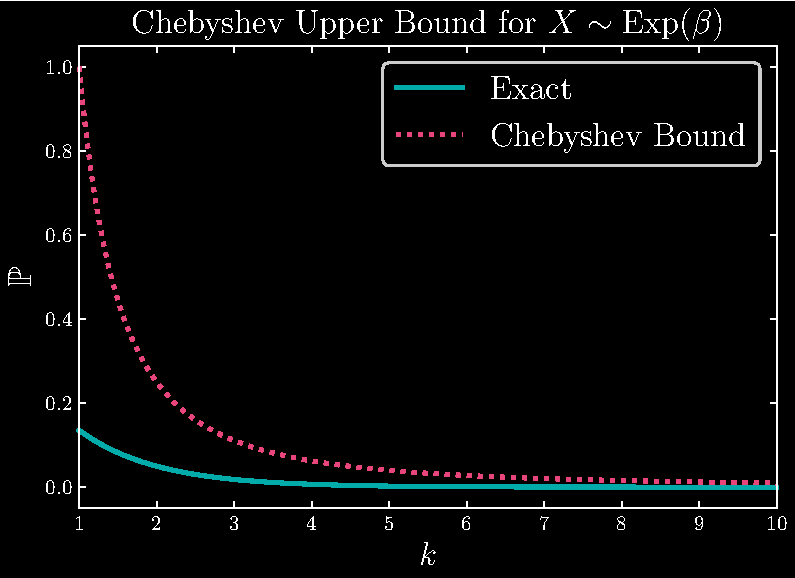
\includegraphics[width=1.0\textwidth]{chap4/chap4ex1.eps}
\end{center}

% QUESTION 2
\qs{4.5.2}{Let \(X \sim \Poisson\left( \lambda  \right)\). Use Chebyshev's inequality to show that \(\Prob\left( X \ge 2 \lambda  \right) \le 1/\lambda \).}
\begin{proof}[Proof] 
For \(X \sim \Poisson\left( \lambda  \right)\), we have \(\mu_{X} = \sigma_{X}^{2} = \lambda \). In the case where \(X - \lambda \ge 0\) and \(t = \lambda \), we have
\begin{align*}
	\Prob\left( \abs{X - \lambda} \ge \lambda \right) & = \Prob\left( X - \lambda \ge \lambda  \right) \\
	 & = \Prob\left( X \ge 2 \lambda  \right) \\ 
\end{align*}
Note that when \(X - \lambda < 0\) with \(t = \lambda \), we have
\begin{align*}
	\Prob\left( \abs{X - \lambda} \ge t \right) & = \Prob\left( -\left( X - \lambda  \right) \ge \lambda  \right)  \\
	 & = \Prob\left( X \le \lambda - \lambda  \right) \\
	 & = \Prob\left( X \le 0 \right) \\
	 & = 0
\end{align*}
so we need only consider the case where \(X - \lambda \ge 0\). Applying Chebyshev's inequality, we can conclude
\[
	\Prob\left( X \ge 2 \lambda  \right) \le \frac{\lambda }{\lambda^{2}} = \frac{1}{\lambda }
\]
\end{proof}

% QUESTION 3
\qs{4.5.3}{Let \(X_{1}, \dots, X_{n} \sim \Bernoulli\left( p \right)\) and \(\overline{X}_{n} = n^{-1} \sum_{i=1}^{n} X_{i}\). Bound \(\Prob\left( \abs{\overline{X}_{n} - p} > \epsilon \right)\) using Chebyshev's inequality and using Hoeffding's inequality. Show that, when \(n\) is large, the bound from Hoeffding's inequality is smaller than the bound from Chebyshev's inequality.}
\begin{proof}[Proof] 
For \(\overline{X}_{n}\), we have \(\E\left( \overline{X}_{n} \right) = p\) and \(\var\left( \overline{X}_{n} \right) = p \left( 1-p \right) / n\). The upper bounds from Chebyshev and Hoeffding are
\begin{align*}
	\Prob\left( \abs{\overline{X}_{n} - p} > \epsilon  \right) & \le \frac{p \left( 1-p \right) }{n \epsilon^{2}} &&\text{(Chebyshev)} \\
	\Prob\left( \abs{\overline{X}_{n} - p} > \epsilon  \right) & \le 2 e^{-2n \epsilon^{2}}  &&\text{(Hoeffding)} \\ 
\end{align*}
Taking the ratio of the Hoeffding to Chebyshev limits, we aim to calculate
\[
	\lim_{n \to \infty} \frac{2 e^{-2n \epsilon^{2}}}{p(1-p) / n \epsilon^{2}} = \frac{1}{p \left( 1-p \right) }\lim_{n \to \infty} \frac{2n \epsilon^{2}}{e^{2n \epsilon^{2}}}
\]
Using l'H\^{o}pital's rule to evaluate the limit since \(\lim_{n \to \infty} 2n \epsilon^{2} = +\infty\) and \(\lim_{n \to \infty} e^{2n \epsilon^{2}} = +\infty\), we have
\[
\frac{1}{p \left( 1-p \right) } \lim_{n \to \infty} \frac{2n \epsilon^{2}}{e^{2n \epsilon^{2}}} = \frac{1}{p \left( 1-p \right)} \lim_{n \to \infty} \frac{2 \epsilon^{2}}{2 \epsilon^{2} e^{2n \epsilon^{2}}} = \frac{1}{p \left( 1-p \right)} \lim_{n \to \infty} \frac{1}{e^{2n \epsilon^{2}}} = 0
\]
ascertaining that Hoeffding is a tighter bound than Chebyshev.
\end{proof}

\newpage
% QUESTION 4
\qs{4.5.4}{Let \(X_{1}, \dots, X_{n} \sim \Bernoulli\left( p \right)\).
\begin{enumerate}[label=(\alph*)]
	\item Let \(\alpha > 0\) be fixed and define
		\[
			\epsilon_{n} = \sqrt{\frac{1}{2n} \log\left( \frac{2}{\alpha } \right)}.
		\]
	Let \(\widehat{p}_{n} = n^{-1} \sum_{i=1}^{n} X_{i}\). Define \(C_{n} = \left(\widehat{p}_{n} - \epsilon_{n}, \widehat{p}_{n} + \epsilon_{n}\right)\). Use Hoeffding's inequality to show that
	\[
		\Prob\left( C_{n} \text{ contains } p \right) \ge 1 - \alpha .
	\]
	In practice, we truncate the interval so it does not go below 0 or above 1.
	\item \textsf{(Computer Experiment.)} Let's examine the properties of this confidence interval. Let \(\alpha = 0.05\) and \(p = 0.4\). Conduct a simulation study to see how often the interval contains \(p\) (called the coverage). Do this for various values of \(n\) between 1 and 10000. Plot the coverage versus \(n\).
	\item Plot the length of the interval versus \(n\). Suppose we want the length of the interval to be no more than \(.05\). How large should \(n\) be?
\end{enumerate}}
\begin{proof}[Proof] 
	(a) Since \(\overline{X}_{n} = \widehat{p}_{n}\) and \(\Prob\left( \abs{\overline{X}_{n} - p} > \epsilon_{n} \right) \le \alpha \), by complementary events (either \(\abs{\overline{X}_{n} - p} > \epsilon_{n}\) or \(\abs{\overline{X}_{n} - p} \le \epsilon_{n}\)), we have
\[
	\Prob\left( \abs{\overline{X}_{n} - p} \le \epsilon_{n} \right) \ge 1 - \alpha 
\]
\end{proof}

\par (b) Here, we sample numerous values of \(\widehat{p}_{n}\), construct \(C_{n}\) from each value, and determine if \(p \in C_{n}\). 

\begin{python}
k, n = 1000, 10000
alpha = 0.05
eps = np.sqrt((1/(2*n))*np.log(2/alpha))
p = 0.4

def confinttest(k,n):
    s = np.random.binomial(1,p,size=(k,n)).mean(axis=1)
    return (p > s - eps) & (p < s + eps);

def coverage():
    coverage = []
    for i in range(1,n+1):
        count = np.count_nonzero(confinttest(k,i) == True)
        coverage.append(count / k)
    return coverage;
\end{python}

\begin{center}
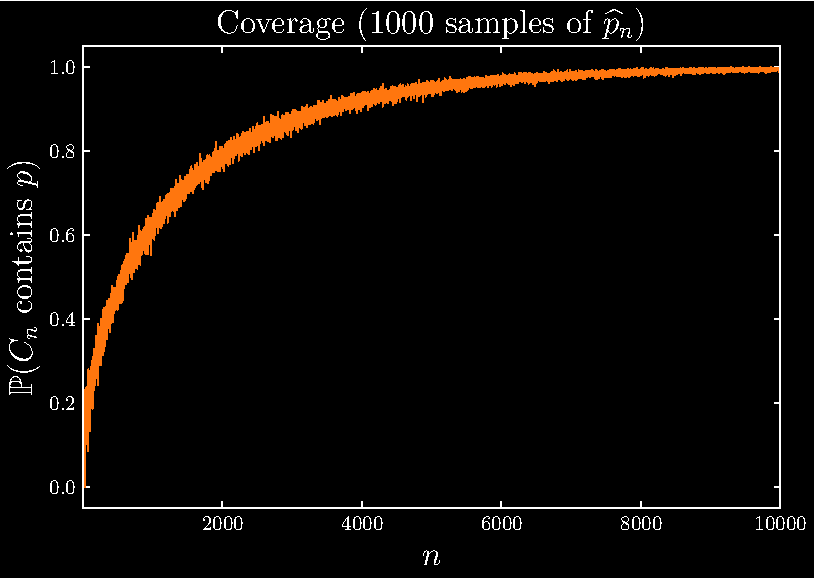
\includegraphics[width=1.0\textwidth]{chap4/chap4ex4b}
\end{center}

As \(n \rightarrow +\infty\), we see that the coverage asymptotically approaches 1. Intuitively this is sensible. Since \(X_{i} \sim \Bernoulli\left( p \right)\), for large \(n\), \(\widehat{p}_{n} \rightarrow p\) (this is the weak law of large numbers, covered in the next chapter). 

\par (c) The length of \(C_{n}\) is \(2 \epsilon_{n}\), and for the length to be no more than \(0.05\), have \(n \ge 2952\).

\begin{python}
def intlength(n):
    epsilons = np.empty(n)
    for i in range(1,n+1):
        epsilon = np.sqrt((1/(2*i))*np.log(2/alpha))
        epsilons[i-1] = 2*epsilon
    return epsilons;

n = 5000
nsolution = np.argwhere(intlength(n) < 0.05).min() + 1
\end{python}

\begin{center}
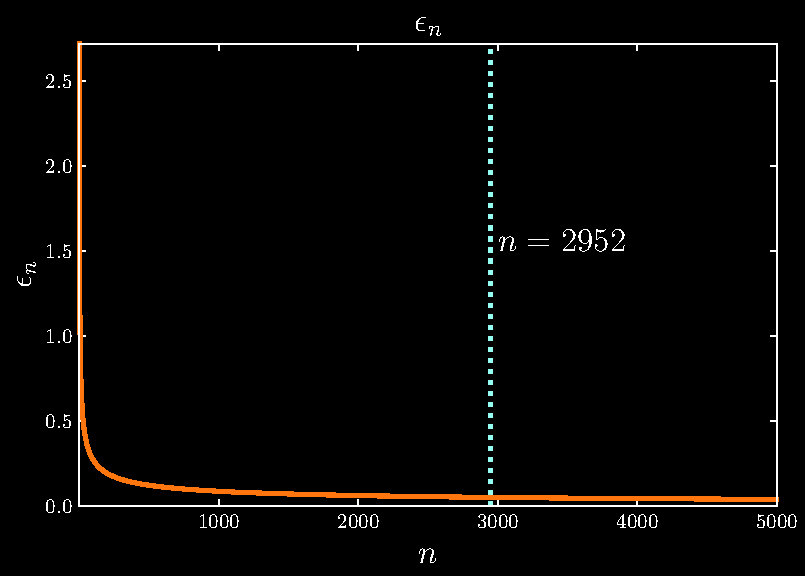
\includegraphics[width=1.0\textwidth]{chap4/chap4ex4c.eps}
\end{center}


% QUESTION 5
\qs{4.5.5}{Prove Mill's inequality, Theorem 4.7. Hint. Note that \(\Prob\left( \abs{Z} > t \right) = 2 \Prob\left( Z > t \right)\). Now write out what \(\Prob\left( Z > t \right)\) means and note that \(x/t > 1\) whenever \(x > t\).}
\thm{(Wasserman 4.7) (Mill's Inequality)}{Let \(Z \sim N \left( 0,1 \right) \). Then
\[
	\Prob\left( \abs{Z} > t \right) \le \sqrt{\frac{2}{\pi }} \frac{e^{-t^{2}/2}}{t}.
\]}
\begin{proof}[Proof] 
By symmetry of the standard normal distribution, 
\[
	\Prob\left( \abs{Z} > t \right) = 2 \Prob\left( Z > t \right)
\] 
Then
\begin{align*}
	\Prob\left( \abs{Z} > t \right) & = 2 \Prob\left( Z > t \right) \\
	 & = 2 \int^{\infty}_{t} \frac{1}{\sqrt{2 \pi }} \exp\left( -\frac{z^{2}}{2} \right) \ dz \\ 
\end{align*}
Now, multiply both sides by \(t\):
\begin{align*}
	\implies t \Prob\left( \abs{Z} > t \right) & = \sqrt{\frac{2}{\pi }} t \int^{\infty}_{t} \exp\left( -\frac{z^{2}}{2} \right) \ dz  \\
	 & \le \sqrt{\frac{2}{\pi }} \int^{\infty}_{t} z \exp\left( -\frac{z^{2}}{2} \right) \ dz  \\ 
	 & = \sqrt{\frac{2}{\pi }} e^{-t^{2}/2}
\end{align*}
which lastly implies that \(\Prob\left( \abs{Z} > t \right) \le \sqrt{\frac{2}{\pi }} e^{-t^{2}/2} / t\).
\end{proof}

% QUESTION 6
\qs{4.5.6}{Let \(Z \sim N \left( 0,1 \right) \). Find \(\Prob\left( \abs{Z} > t \right)\) and plot this as a function of \(t\). From Markov's inequality, we have the bound \(\Prob\left( \abs{Z} > t \right) \le \frac{\E\left| Z \right|^{k}}{t^{k}}\) for any \(k>0\). Plot these bounds for \(k = 1,2,3,4,5\) and compare them to the true value of \(\Prob\left( \abs{Z} > t \right)\). Also, plot the bound from Mill's inequality.}

Some initial observations to bear in mind:
\begin{itemize}
	\item Observe that \(\Prob\left( \abs{Z} > t \right)\) is the two-tailed probability that we observe \(Z > t\), when \(Z \ge 0\), or \(Z < -t\), when \(Z < 0\).
	\item Using Markov's inequality, \(\Prob\left( \abs{Z} > t \right) = \Prob\left( \abs{Z}^{k} > t^{k} \right) \le \E \abs{Z}^{k} / t^{k} \). 
	\item The expectation term \(\E\left( \abs{Z} \right)\) is defined as
\[
	\E \abs{Z} = \int^{+\infty}_{0} z f_{Z}\left( z \right) \ dz + \int^{0}_{-\infty} z f_{Z}\left( z \right) \ dz = 2 \int^{+\infty}_{0} z f_{Z}\left( z \right) \ dz = \sqrt{\frac{2}{\pi }} 
\]
\end{itemize}

Running a horse race between the exact two-tail probability and the Markov and Mill bounds, we find:

\begin{python}
def normtest(t): 
    normal_dist = norm(0,1)
    domain = np.arange(0,t+0.01,0.01)
    probs = np.empty(len(domain))
    for i, j in zip(domain, range(0, len(domain))):
        probs[j] = (2*(1-normal_dist.cdf(i)))
    return probs;

def markov(k, t):
    domain = np.arange(0.01,t+0.01,0.01)
    markovs = np.empty(len(domain))
    exptabszk = np.power(
    		np.absolute(np.random.normal(0,1,1000)), k).mean()
    for i, j in zip(domain, range(0, len(domain))):
        markovs[j] = np.divide(exptabszk, np.power(i,k))
    return markovs;

def mill(t):
    domain = np.arange(0.01,t+0.01,0.01)
    mills = np.empty(len(domain))
    for i, j in zip(domain, range(0, len(domain))):
        mills[j] = np.sqrt(2 / math.pi)*(np.exp(-np.square(i)/2)/i)
    return mills;

t = 5.5
\end{python}

\begin{center}
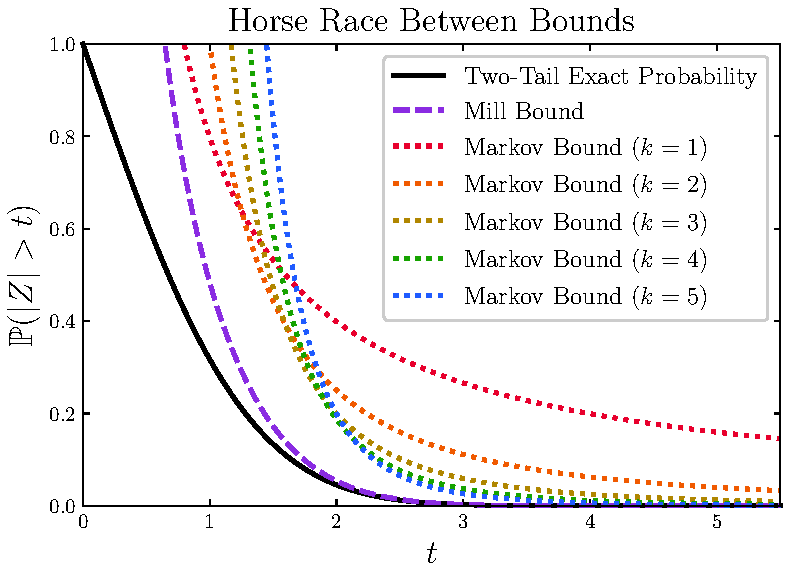
\includegraphics[width=1.0\textwidth]{chap4/chap4ex6.eps}
\end{center}

% QUESTION 7
\qs{4.5.7}{Let \(X_{1}, \dots, X_{n} \sim N \left( 0,1 \right) \). Bound \(\Prob\left( \abs{\overline{X}_{n}} > t \right)\) using Mill's inequality, where \(\overline{X}_{n} = n^{-1} \sum_{i=1}^{n} X_{i}\). Compare to the Chebyshev bound.}
First note that \(\E\left( \overline{X}_{n} \right) = 0\) and \(\var\left( \overline{X}_{n} \right) = 1/n\). Thus \(\overline{X}_{n} \sim N \left( 0, 1/n \right) \). In order for Mill's inequality to be applicable, we transform \(\overline{X}_{n}\) and \(t\) to be standard normal:
\begin{align*}
	\Prob\left( \left|\frac{\overline{X}_{n}}{\sqrt{1/n}} \right| > \frac{t}{\sqrt{1/n}}\right) & = \Prob\left( \left|\frac{\overline{X}_{n}}{\sqrt{1/n}} \right| > \sqrt{n}t \right)  \\
	 & \le \sqrt{\frac{2}{\pi }} \frac{e^{- \left( \sqrt{n}t \right)^{2} / 2}}{\sqrt{n} t} \\ 
	 & = \sqrt{\frac{2}{n \pi }} \frac{e^{-nt^{2}/2}}{t}
\end{align*}

And Chebyshev's inequality is given simply by
\[
	\Prob\left( \abs{\overline{X}_{n}} \ge t \right) \le \frac{1}{n t^{2}}
\]
Taking the limit of the ratio of the Mill bound to the Chebyshev for large \(n\) gives us
\[
	\lim_{n \to \infty} \frac{\sqrt{\frac{2}{ n \pi}} \frac{e^{-nt^{2}/2}}{t}}{1 / nt^{2}} = \lim_{n \to \infty} \sqrt{\frac{2n}{\pi }} t e^{-nt^{2}/2} = \boxed{0}
\]
yielding the conclusion that Mill is a smaller bound than Chebyshev.
	

\end{document}
